\documentclass[10pt,twocolumn,letterpaper]{article}
 \pdfoutput=1
\usepackage{cvpr}
\usepackage{times}
\usepackage{epsfig}
\usepackage{graphicx}
\usepackage{amsmath}
\usepackage{amssymb}
\usepackage{bm}
%\usepackage{subcaption}
%\usepackage{slashbox}
\usepackage{color}
\usepackage[english]{babel}
%\usepackage[linesnumbered,ruled,vlined]{algorithm2e}
\usepackage[breaklinks=true,bookmarks=false]{hyperref}
\usepackage{booktabs}
\usepackage{caption}
\usepackage{algorithm}
\usepackage{algorithmic}

\DeclareCaptionLabelFormat{noname}{#2}
\captionsetup[algorithm]{labelformat=noname}

\newlength\myindent
\setlength\myindent{2em}
\newcommand\bindent[1][\myindent]{%
  \begingroup
  \setlength{\itemindent}{#1}
  \addtolength{\algorithmicindent}{#1}
}
\newcommand\eindent{\endgroup}


\usepackage{multirow}
\newcommand{\ra}[1]{\renewcommand{\arraystretch}{#1}}

\newcommand{\argmin}{\operatornamewithlimits{argmin}}
\cvprfinalcopy

\def\cvprPaperID{16} % *** Enter the CVPR Paper ID here
\def\httilde{\mbox{\tt\raisebox{-.5ex}{\symbol{126}}}}
\begin{document}
\title{DeepAutoTrack (DAC): Car Trajectory Prediction for Autonomous Driving}

\author{Di Wu, Zhennan Wang, Yi Tang,  Wenbin Zou, Xia Li\\
Shenzhen University\thanks{Shenzhen Key Lab of Advanced Telecommunication and Information Processing, College of Information Engineering, Shenzhen University.}\\
{\tt\small dwu,...@szu.edu.cn}}
\maketitle
%%%%%%%%% ABSTRACT
\begin{abstract}
TODO: abstract
This guide is patterned after my �Doing well in your courses�, a post I wrote a long time ago on some of the tips/tricks I�ve developed during my undergrad. I�ve received nice comments about that guide, so in the same spirit, now that my PhD has come to an end I wanted to compile a similar retrospective document in hopes that it might be helpful to some. Unlike the undergraduate guide, this one was much more difficult to write because there is significantly more variation in how one can traverse the PhD experience. Therefore, many things are likely contentious and a good fraction will be specific to what I�m familiar with (Computer Science / Machine Learning / Computer Vision research). But disclaimers are boring, lets get to it!
\end{abstract}
%%%%%%%%% BODY TEXT
%%% Andrje Karpathy's blog: http://karpathy.github.io/2016/09/07/phd/
%%% Another great resource on this topic is Tips for Writing Technical Papers from Jennifer Widom.
%%% https://cs.stanford.edu/people/widom/paper-writing.html
\section{Introduction}


\begin{figure}

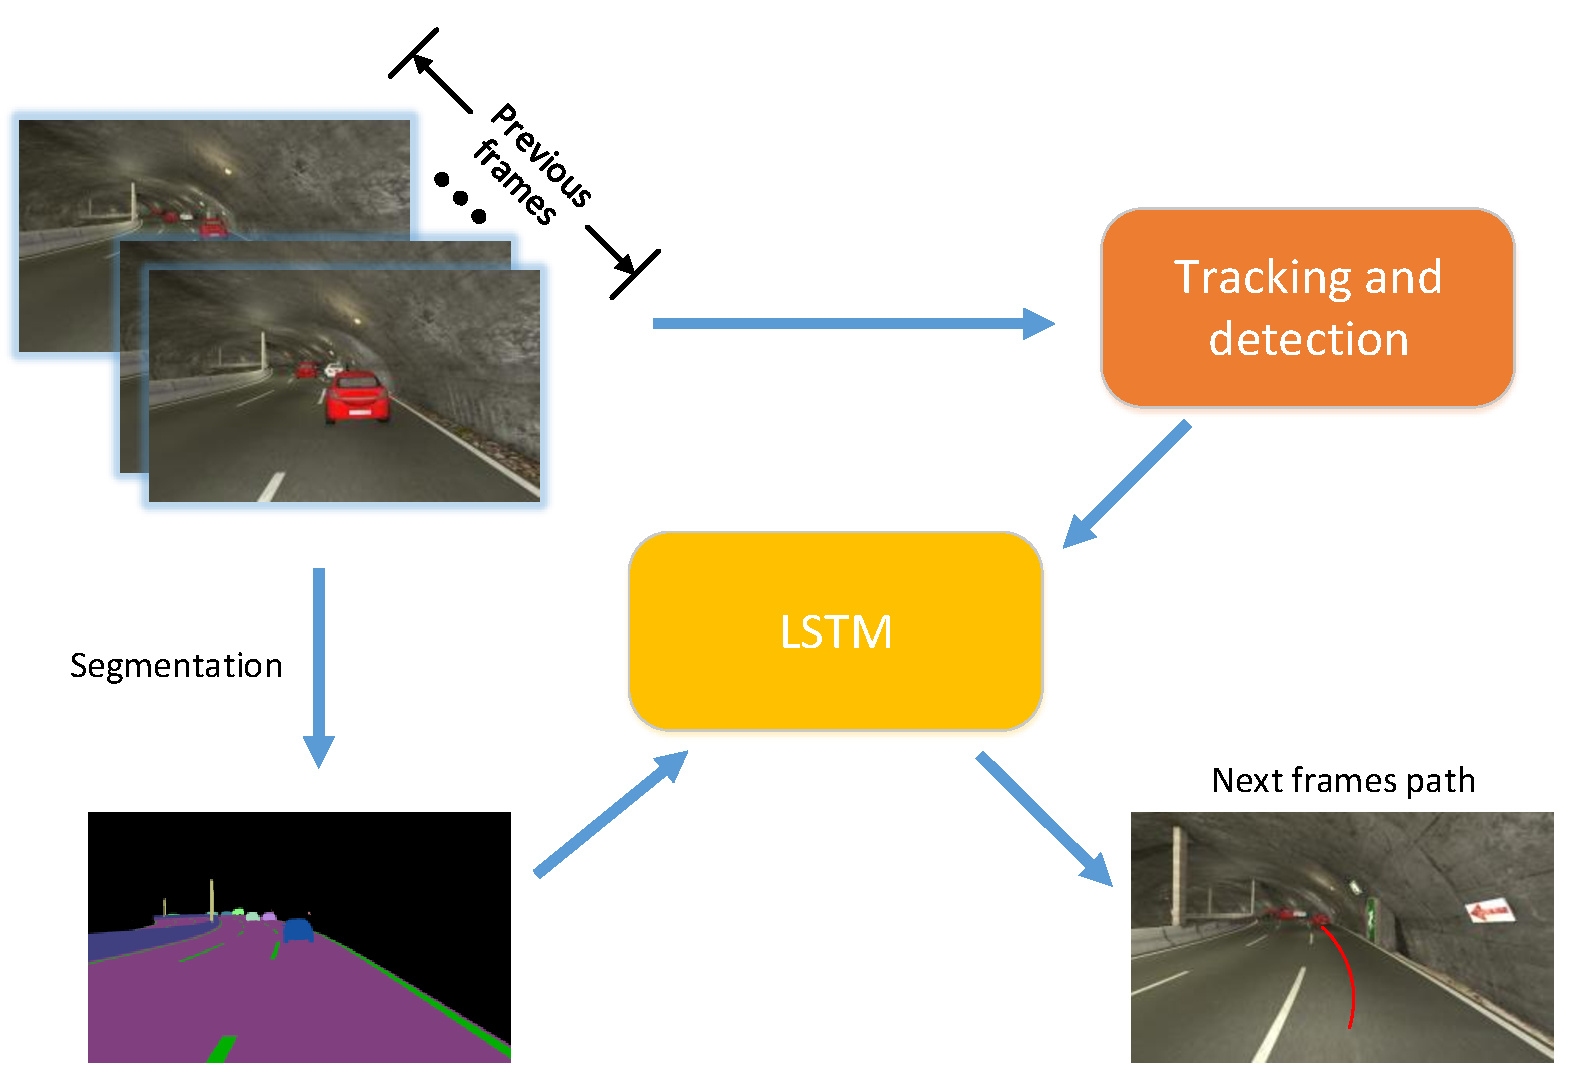
\includegraphics[width=8.8cm]{pool_figure}
\caption{pool figure}
\label{figure10}
\end{figure}



\textbf{\emph{1. What is the problem?}}

Currently, there are two major paradigms for autonomous driving systems built upon vision-based input~\cite{chen2015deepdriving}: mediated perception approaches that firstly explain the vision input and than parse the scene to make a driving policy (usually by a controller with if-then-else rules), and behaviour reflex approaches that directly map the vision input to a driving policy by a regressor.

In this paper, in the framework of first paradigm, we try to tackle the problem of predicting future trajectories of cars given its past information.

\textbf{\emph{2. Why is it interesting and important?}}

Driver reaction time is a crucial factor for a human driver to react to the traffic participants. Driver reaction time includes recognising the light has changed, deciding to continue or brake, and if stopping engaging the brake (remove foot from accelerator and apply brake). Accident reconstruction specialists commonly use 1.5 seconds~\cite{mcgehee2000driver}.
Therefore, the ability to predict traffic participants' \emph{future} trajectory will greatly benefits the mediated perception approach's driving policy decision making.

\begin{figure}[t]
        \centering
        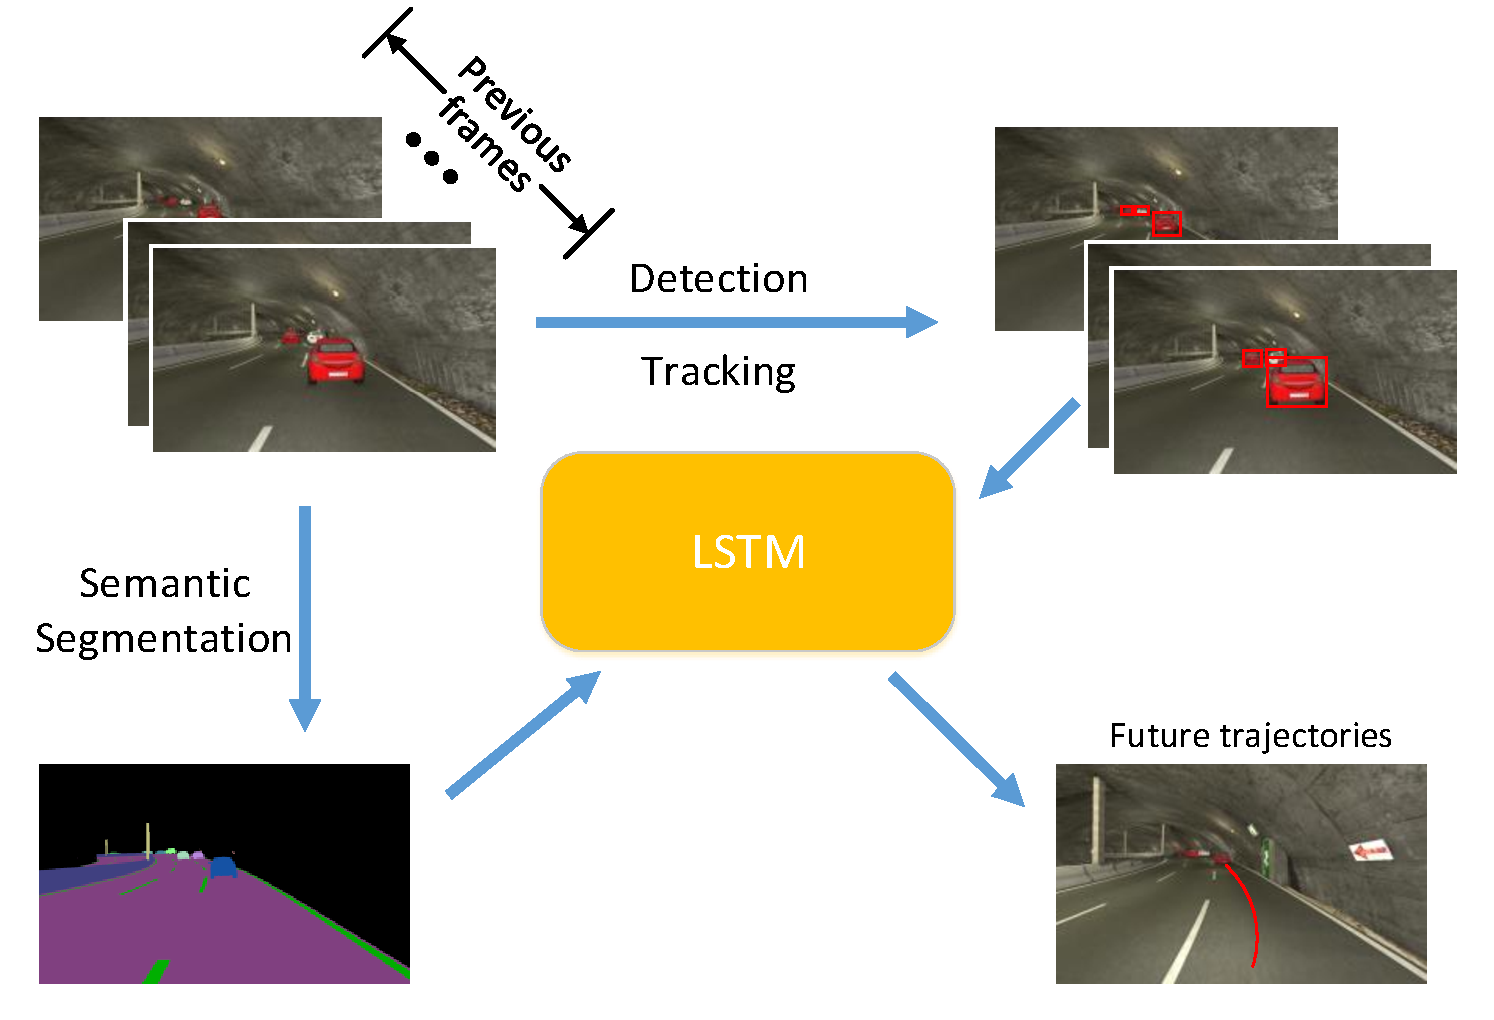
\includegraphics[width=0.45\textwidth]{figures/pull_figure.pdf}
        \caption{ {\small TODO: Pull figure caption goes here.}}
        \label{fig:pull_figure}
\end{figure}
\textbf{\emph{3. Why is it hard? (E.g., why do naive approaches fail?)}}

Individually, for computer vision community, it's an unsolved problem. e.g.: object detection, semantic segmentation, instance segmentation, etc.


Currently, most work focus on static images. However, autonomous driving is intrinsically a dynamic problem. Human driver makes decision by sequence of input frames instead of simply one static frame.

\textbf{\emph{4. Why hasn't it been solved before? (Or, what's wrong with previous proposed solutions? How does mine differ?)}}

Scene parsing results contains quite some spurious information.

In traditional vision based tracking problems (\emph{e.g.} ~\cite{wu2013online, wu2015object, mueller2016benchmark}) where target objects go through rather sporadic movements (usually the object trajectory is generated by artificial movement of the target in order to test the robustness of the tracker), the prediction of target's future trajectory is simply a moot problem.
However, traffic participants generally exhibit regular trajectories (e.g., cars driving on the road and pedestrian walking on the sidewalks).

Currently research community lacks proper evaluation metrics for deciding the temporally future prediction result.



\textbf{\emph{5. What are the key components of my approach and results? Also include any specific limitations.}}

In our approach, there are three key components: traffic participants detection, instance tracking and future trajectory prediction.

% Then have a final paragraph or subsection: "Summary of Contributions". It should list the major contributions in bullet form, mentioning in which sections they can be found. This material doubles as an outline of the rest of the paper, saving space and eliminating redundancy.

Our contributions are as follows:
\begin{itemize}

\item We verify the feasibility of predicting the future trajectories of cars for assisting mediated perception framework. The proposed system stems from the issue of human driver reaction time in the autonomous driving context.

\item We present a novel ``tracking-by-detection" framework in the context of autonomous driving for robustly vehicle tracking. The proposed framework greatly enhanced the trackers' robustness by updating tracker's target representation, in the meanwhile solving the problem of instance association between frames.

\item We design various temporal models for the problem of predicting future trajectories based on historical data and show that the temporal model generating intermediate output utilising the whole historical data performs better than the frame-to-frame based output temporal model.

\item We demonstrate the effectiveness of using ``privileged information"(e.g., scene semantics and car pose information) further boost the prediction accuracy. [NOT DONE YET].

\item We formalise the car trajectory problem into a 3D occupancy grid problem given depth information.

\item We construct a time-series dataset for car trajectory prediction based on the SYNTHIA dataset~\cite{ros2016synthia}.

\end{itemize}



\section{Related Work}

%%% TY: write related work for object detection, segmentation, instance segmentation
\textbf{\emph{1. Object detection, segmentation, instance segmentation}}

TODO: TY
%%% DW: write related work for visual tracking
%%% DW: write related dataset for autonoumous driving
Object detection is an important component in our system. Before the resurgence of convolutional neural network (CNN), Deformable Part Model (DPM) \cite{felzenszwalb2008discriminatively} and Selective Search \cite{Uijlings2013Selective} are the trend of this field. However, after the proposal of R-CNN \cite{girshick2014rich}, which combines Selective Search and deep learning features to detect objects, the architecture of CNN has attracted more attention. At the beginning, R-CNN is a step-by-step and inefficient method. Then, SPPNet \cite{He2015Spatial} exploits a spatial pyramid pooling layer to extract multi-scale deep features and Fast R-CNN \cite{Girshick2015Fast} introduces the multi-task learning to fine-tune all layers in their network. At last, Faster R-CNN \cite{Ren2015Faster} proposes a region proposal network (RPN) and integrates RPN and Fast R-CNN to build a end-to-end architecture. Meanwhile, SSD \cite{liu2016ssd} uses a series of boxes and directly gives the probability for each object class. In addition, YOLO \cite{redmon2016you} proposes a fast object detection method, which divides the input image into grids, then predicts object positions and confidences for each category in each grid.

At the field of semantic segmentation, many methods with CNN also bring a dramatic improvement. FCN \cite{long2015fully} firstly transfers the fully-connected layers into convolution layers, which turns segmentation task into pixel-wise classification task. Deeplab \cite{chen2016deeplab} considers the limitation of receptive field of CNN, and then proposes a dilated convolution layer to solve this problem. DRN \cite{yu2017dilated} further proposes a semantic network by integrating residual structure and dilated convolution. With the modification of neural network, conditional random field (CRF) is employed into refining the output of network in \cite{chen2016deeplab}. After that, CRF is merged into neural network to become an end-to-end architecture \cite{liu2015semantic,zheng2015conditional,arnab2016higher}

\textbf{\emph{2. Visual trackers}}


TODO: DW


%% DW: (1)traditional segmentic segmentation dataset
%% DW: (2) synthetic dataset
%% DW: (3) temporal consistent dataset

\textbf{\emph{3. Dataset for autonoumous driving}}

Camvid dataset~\cite{Camvid} consists of a set of monocular images taken in Cambridge UK. However, only 701 images contain pixel-level annotations over a total of 32 categories (combining objects and architectural scenes).

Similarly, Daimler Urban Segmentation dataset~\cite{scharwachter2013efficient} contains 500 fully labelled monochrome frames for 5 categories.

KITTI benchmark suite~\cite{Geiger2013IJRR} provides a large a mount of images of urban scene from Karlsruhe, Germany, with ground truth data for odometry, object detection, tracking, scene flow and stereo benchmarks. However, a limited 430 labelled images are provided for semantic segmentation.

A common limitation of the aforementioned datasets is the bias introduced by the acquisition of images in a specific city. The LabelMe~\cite{russell2008labelme} project offers the solution by offering around 1,000 fully annotated images of urban environments around the world and more than 3,000 images with partial(noisy) annotations.

More recently, larger project are constructed:
Cityscapes dataset~\cite{Cordts2016Cityscapes} which consists of a collection of images acquired in 50 cities around Germany, Switzerland and France in difference seasons, and having 5,000 images with fine annotations and 20,000 with coarse annotations over a total of 30 classes.

The use of synthetic data has increased considerably in recent years within computer vision community. ~\cite{mueller2016benchmark} provides a synthetic dataset generation and online tracker evaluation. In~\cite{kaneva2011evaluation}, the authors used a photorealistic virtual world to evaluate the performance of image features under scene changes and image transformations. Synthetic data has also been used for skeleton joints estimation~\cite{shotton2013real}, allowing the classifier invariant to pose, body shape, clothing, etc.

A fine annotated images in Cityscape dataset requires on average 1.5 hours which is very labor intensive. Thus, the cost of scaling large project would required a prohibitive economic investment in order to capture images from a larger variety of countries, in different seasons and different traffic conditions. For these reasons, a novel synthetic dataset of urban scene called SYNTHIA~\cite{ros2016synthia} is proposed to use synthetic imagery that simulate real urban scenes in a vast variety of conditions and produce the appropriate annotations.
This dataset is a large collection of images with high variability due to changes in illumination, textures, pose of dynamic objects and camera view-points.

%%% ZN: write related works for Recurrent Networks (used in the context of autonomous driving)
\begin{figure*}[t]
        \centering
        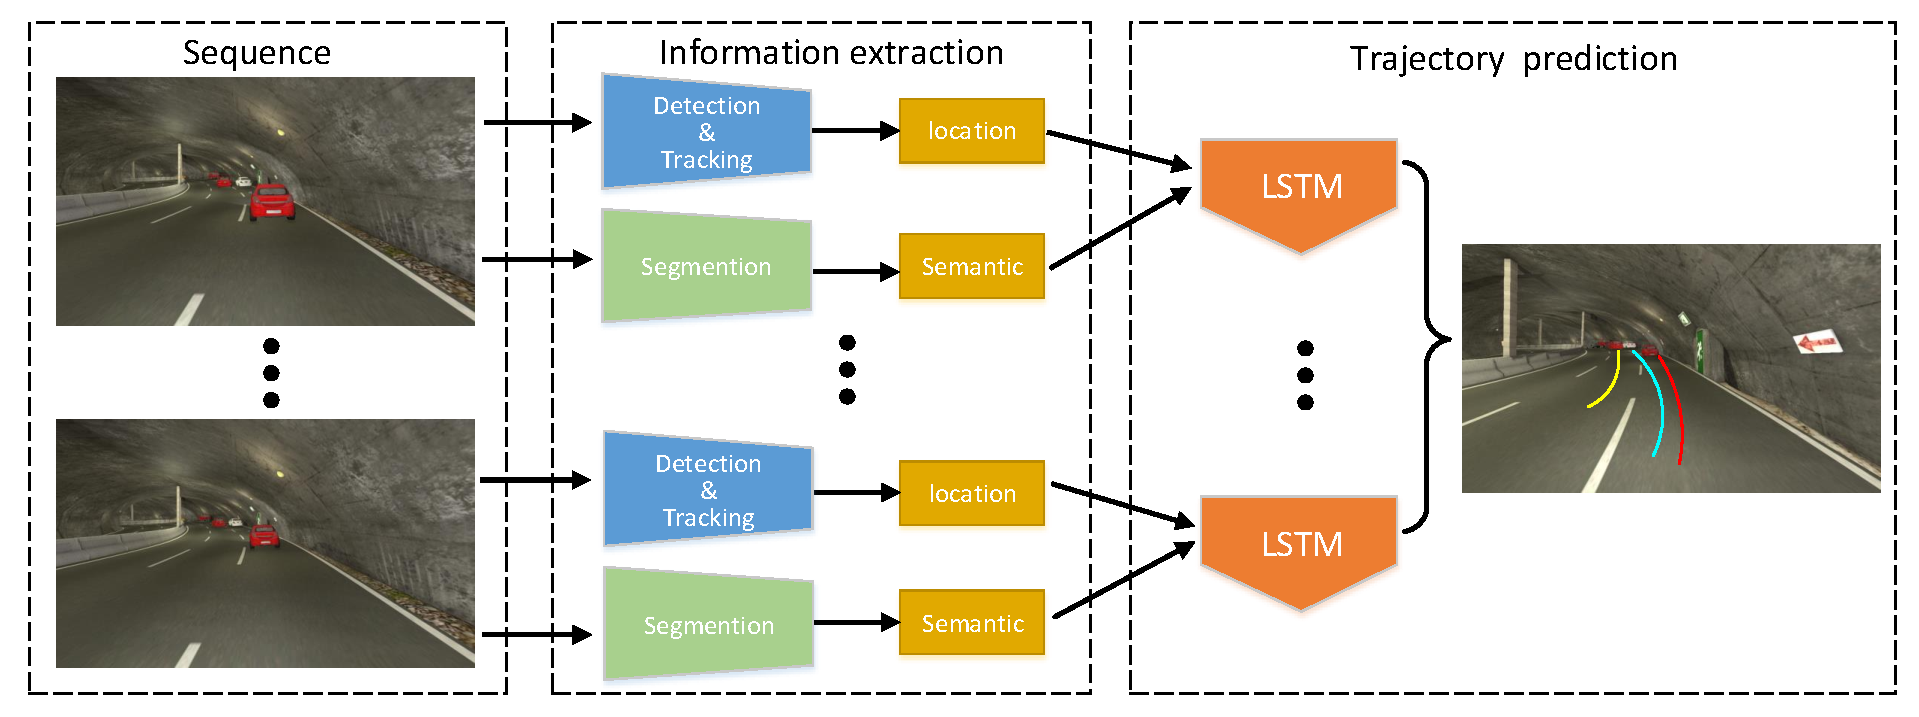
\includegraphics[width=0.75\textwidth]{figures/framework.pdf}
        \caption{ {\small TODO: framework caption goes here.}}
        \label{fig:framework}
\end{figure*}

\textbf{\emph{4. Recurrent Networks (used in the context of autonomous driving)}}



Recently, RNN(recurrent network) and its variant LSTM(long short-term memory) have been successfully used in autonomous driving, due to its advantages for modeling sequential data in vision problems. Most of these works exploit LSTM as component of an end-to-end driving model. ~\cite{xu2017end} used the combination of a fully-convolutional network and an LSTM to learn from large-scale vehicle action data, to predict future egomotion including multi-modal discrete and continuous driving behaviors. ~\cite{kim2017interpretable} used a LSTM network to predict the inverse turning radius and generate a heat map of attention at each timestep conditioned on the previous hidden states and a current convolutional feature cube. ~\cite{duself} used 3D convolutional layers to extract visual features, then fed them into LSTM layers to capture the sequential relation. In addition to using deep features, ~\cite{koutnik2013evolving} trained a large recurrent neural network using a reinforcement learning approach to map images directly to steering angles, with the purpose to keep the car on track.

TODO: cite below papers;

~\cite{xu2017end}: End-to-end learning of driving models from large-scale video dataset.

~\cite{behl2017bounding} Bounding Boxes, Segmentations and Object Coordinates: How Important is Recognition for 3D Scene Flow Estimation in Autonomous Driving Scenarios?

~\cite{chen2015deepdriving} DeepDriving: Learning Affordance for Direct Perception

~\cite{kim2017interpretable} Interpretable Learning for Self-driving cars


\section{Proposed Algorithm}

We first describe our overall approach for car trajectory prediction and the details of implementation are presented in Sec~\ref{sec:Implementations}.
Our goal is via collecting the visual information from the past to predict the traffic participants future trajectory. Fig.~\ref{fig:framework} shows the overall architecture of our proposed framework.

\subsection{Traffic Participants detection}


\subsection{Instance tracking}

We compare two state-of-the-art trackers (given the time vs. accuracy) of the trackers.
\begin{figure}[t]
        \centering
        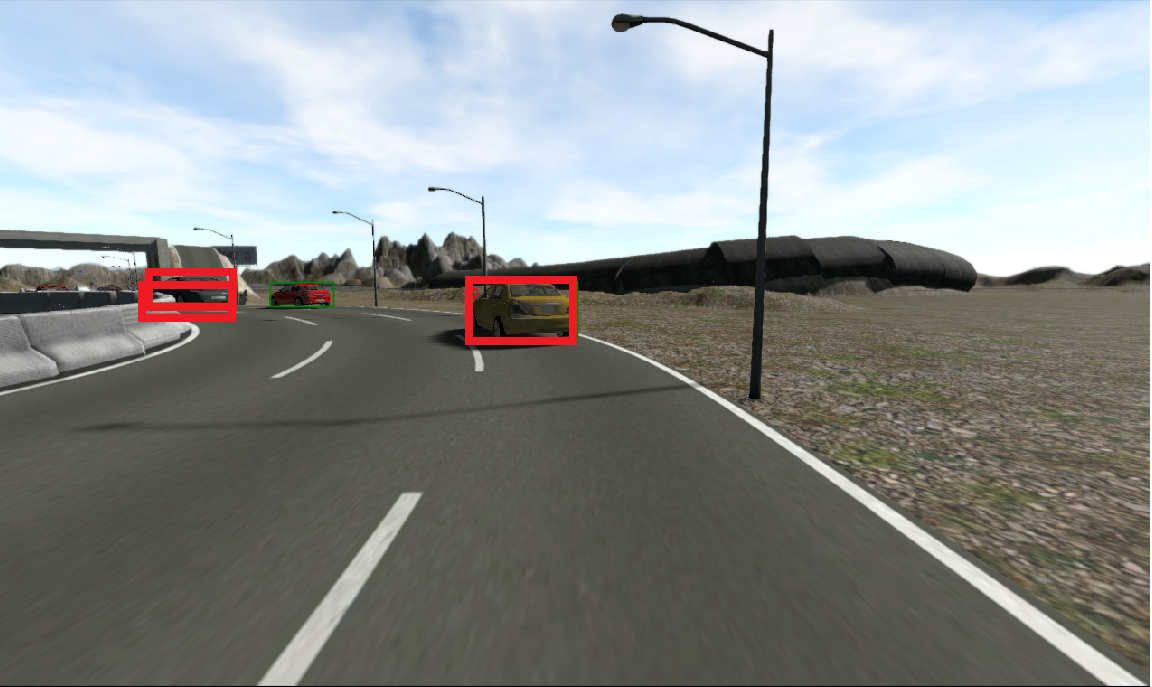
\includegraphics[width=0.4\textwidth]{figures/double_detection.png}
        \caption{ {\small TODO: Instance association caption goes here.}}
        \label{fig:Instance_associationn}
\end{figure}

\subsection{Semantic segmentation}
We use the state-of-the-art semantic segmentation networks: Dilated Residual Networks (DRN)~\cite{yu2017dilated}.

\subsection{Trajectory prediction}


We compare two temporal models based on LSTM cells for predicting the car trajectory.

%%%%%%%%%%%%%%%%%%%%%%%%%%%%%%%%%%%%%%%%%%%%%%%%%%%%%%%%%%%%%%%%%%%%%%%%%%%%%%%%%%%%%%%%%%%%%%%%%%%%%%%%%%%
\section{Experiments}

\subsection{Dataset collection}

Currently, most public datasets with semantic labelling are single frame, static images. Continuous video streams are required for the purpose of car trajectory prediction.
We collect car trajectory prediction dataset based on the SYNTHIA~\cite{ros2016synthia} dataset.
SYNTHIA dataset is a large corpus of synthetic images originally collected for the purpose of semantic segmentation of urban scenes generated by rendering a virtual city created with the Unity development platform.
The potential of this virtual world includes extension capabilities: new parts of the cities and road conditions can be easily generated by adding different setups. The major features of collected dataset include: scene diversity (European style town, modern city, highway and green areas), variety of dynamic objects (cars, pedestrians and cyclists), multiple seasons (dedicated themes for winter, fall, spring and summer), lighting conditions and weather (dynamic lights and shadows, several day-time modes, rain mode and night mode).
There are more than 200,000 HD ($760\times1280$) photo-realistic frames from video streams.
Frames are acquired from multiple view-points (up to eight views per location), and each of the frames also contains an associated depth map. In our experiment, we used only left front camera view data.

The focus of this paper is on car trajectory prediction on high ways which corresponds to sequence number 1 in the SYNTHIA dataset. We especially concern about the cars that are relatively close to the driver. Hence, we start tracking the vehicle when the vehicle's pixel occupancy rate \emph{(POR)} is larger than 0.2\% and stop tracking the instance when the POR is smaller than 0.1\%. The POR of 0.2\% and 0.1\% correspond to roughly 30 and 50 meters of relative distance between the driver and tracking vehicle so as to suffice the safety distance for drivers to make timely reaction.
We follow the traditional paradigm for tracking to collect target's bounding box: $[x, y, w, h]$ of each frame. Moreover, the minimum relative distance $d_{min}$ and maximum relative distance $d_{max}$ can also be acquired from the depth camera.
We list our logic for collecting continuous car tracking in List~\ref{list:dataset_collection}.
Some sample frames with its sementic labels and depth information is shown in Fig. (TODO: TY help to generate the figures).

TODO: generate a table for total number of frames and sequence tracklets!

\begin{algorithm}[h]
\begin{algorithmic}
\caption{\textbf{Dataset ground truth construction}}\label{list:dataset_collection}
\STATE \textbf{Step 1} $\rightarrow $ get traffic participants from ground truth annotation with only cars as instances.
\STATE \textbf{Step 2} {$\rightarrow $ {
\bindent
  \IF{POR $> 0.2\%$}
    %\bindent[1.45cm]
    \STATE $\Rightarrow$ start tracking instance ,
    \STATE $\Rightarrow$ collecting 3D tracking rectangular: $[x, y, w, h, d_{min}, d_{max}]$
    \STATE $\Rightarrow$ collecting semantic segmentation image, $I_{seg}$.
    \STATE $\Rightarrow$ collecting 2d car pose from RGB input $I_{car}$.
    %\eindent
  \ELSIF{POR $< 0.1\%$}
    \STATE $\Rightarrow$ stop tracking
    \ENDIF\eindent}
  }
\STATE \textbf{Step 3} $\rightarrow $ split sequences into tracklets of 23 frames:
{\bindent
    \STATE $\Rightarrow$  first 15 frames (5Hz, 3 sec) as training input
    \STATE $\Rightarrow$  next 8 frames (1.6 sec) as the held-up future trajectory to be predicted.
\eindent}
\end{algorithmic}
\end{algorithm}
%%%%%%%%%%%%%%%%%%%%%%%%%%%%%%%%%%%%%%%%%%%%%%%%%%%%%%%%%%%%%%%%%%%%%%%%%%%%%%%%%%%%%%%%%%%%%%%%%%%%%%%%%%%%%%%%

\subsection{Implementations}\label{sec:Implementations}

\begin{table*}\centering
\ra{1.}
\begin{tabular}{@{}llllllllllll@{}}\toprule
\multicolumn{2}{c}{conf}  & 0.5  & 0.55 & 0.6 &  0.65 & 0.7  & 0.75 & 0.8 &  0.85 & 0.9  & 0.95\\
\hline
\multirow{3}{*}{SSD}&   precision & \textbf{92.0 } & 91.8 & 91.7 & 91.4 & 91.1 & 91.0 & 90.5 & 90.2 & 89.4 & 87.4\\
                    &    recall   & \textbf{92.3}  & 92.1 & 92.0 & 91.8 & 91.4 & 91.3 & 90.8 & 90.5 & 89.7 & 87.7\\
                    &    f-score  & \textbf{92.2 } & 92.0 & 91.8 & 91.6 & 91.3 & 91.1 & 91.1 & 90.4 & 89.6 & 87.6\\
\multirow{3}{*}{Faster-RCNN}
                    &   precision & 81.2  & 81.2  & 81.1 & 81.1 & 81.1 & 81.0 & 81.0 & 80.7 & 80.5 & 80.0 \\
                    &   recall    & 91.4  & 91.4  & 91.3 & 91.3 & 91.3 & 91.3 & 91.3 & 90.9 & 90.7 & 90.2\\
                    &   f-score   & 86.0  & 86.0  & 86.0 & 86.0 & 86.0 & 86.0 & 86.0 & 85.5 & 85.3 & 84.8\\
\bottomrule
\end{tabular}
\caption{Caption: TODO results: (1) SSD better at detecting large object(which is in our case). (2) Faster-RCNN  is more robust to confidence threshold}
\label{tab:ssd_fasterrcnn}
\end{table*}
\subsubsection{Traffic participants detection}

We compared two state-of-the-art approaches: SSD~\cite{liu2016ssd} and Faster-RCNN~\cite{ren2015faster} for detecting the traffic participants.
We use the pretrained network on the PASCAL VOC detection dataset~\cite{everingham2015pascal} which has 20 classes and fine-tune the network on the SYNTHIA with two classes: cars \emph{v.s.} background.
A comprehensive survey of trade-offs for modern convolutional object detectors is presented in~\cite{huang2017speed} and we refer keen readers to the aforementioned paper for a more complete comparison to achieve the right speed/memeory/accuracy balance for a given application and platform.

As it is also pointed out in the paper~\cite{huang2017speed} that SSD, albeit is less advantageous in detecting small object, it's very competitive for detecting larger objects. In this paper, we concerns mostly about cars that are closer to the driver. Hence, we chose the POR as 0.2\% which favors detectors that are robust in larger object detection.
Tab.~\ref{tab:ssd_fasterrcnn} also verifies that SSD is indeed more competitive when the objects of interest are large.

\subsubsection{Instance tracking}

We compare two state-of-the-art trackers (given the time vs. accuracy) of the trackers.

\subsubsection{Trajectory prediction}

We compare two temporal models based on LSTM cells for predicting the car trajectory.

%%%%%%%%%%%%%%%%%%%%%%%%%%%%%%%%%%%%%%%%


\subsection{Evaluation}
\begin{figure}[t]
        \centering
        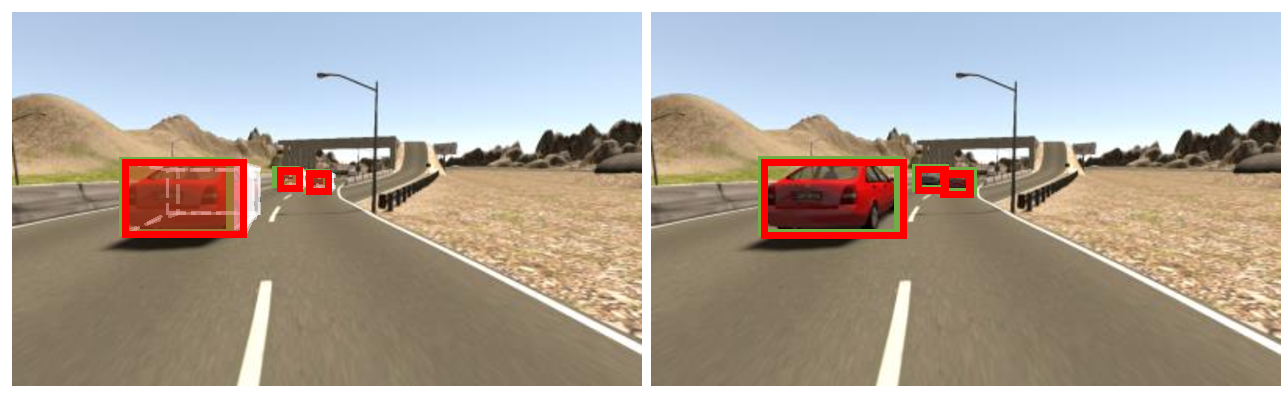
\includegraphics[width=0.5\textwidth]{figures/evaluation.pdf}
        \caption{ {\small TODO: evaluation caption goes here.}}
        \label{fig:evaluation}
\end{figure}

\begin{table}[t]
\small
   \centering
        \begin{tabular}{|l|| *{2}{c}| *{2}{c} |}\hline
            {\small Configuration} & \multicolumn{2}{|c|}{\small 2D}  & \multicolumn{2}{|c|}{\small 3D}  \\ \hline \hline
                                                    & P20       & AUC       & P20       & AUC  \\ \hline \hline

            {\small MTM }                          &  58.0     &  38.4     & 64.3      & 44.0   \\
            \hline
            {\small \textbf{MTFC} }  &  66.2 ${\color{red}(8.2\uparrow)}$    &  46.1 ${\color{red}(7.7\uparrow)}$    &  71.4 ${\color{red}(7.1\uparrow)}$     &  49.1 ${\color{red}(5.1\uparrow)}$\\
            \hline
            \hline
            {\small MaxRes }                        &  57.5     &  38.8     &  65.8     &  45.9  \\
            \hline
            {\small \textbf{MTM (GT)} }        &  70.6${\color{red}(13.1\uparrow)}$     &  46.7  ${\color{red}(7.9\uparrow)}$   &  77.8 ${\color{red}(12.0\uparrow)}$    &  53.6 ${\color{red}(7.7\uparrow)}$ \\
            \hline
            \hline
            {\small \textbf{MTFC}}           &  74.0${\color{red}(3.4\uparrow)}$      &  51.8${\color{red}(5.1\uparrow)}$      &  79.8${\color{red}(2.0\uparrow)}$      &  57.0${\color{red}(3.4\uparrow)}$    \\
            \hline
            {\small \textbf{DAC}}&  74.2 ${\color{red}(0.2\uparrow)}$    &  52.1${\color{red}(0.3\uparrow)}$     &  79.9${\color{red}(0.1\uparrow)}$     &  57.4${\color{red}(0.4\uparrow)}$\\\hline

        \end{tabular}

    \caption{ {\small
         TODO: this table is just a place holder, currently has no meaning.}
          } \label{table_baseline}
\end{table}


\begin{table}[t]
\small
   \centering
        \begin{tabular}{|l|| *{2}{c}|}\hline
            {\small Configuration} & \multicolumn{2}{|c|}{\small 2D}    \\ \hline \hline
                                                  & P20       & AUC   \\ \hline \hline

            {\small MTM }                          &  58.0     &  38.4      \\
            \hline
            {\small \textbf{MTFC} }  &  66.2 ${\color{red}(8.2\uparrow)}$    &  46.1 ${\color{red}(7.7\uparrow)}$  \\
            \hline
            \hline
            {\small MaxRes }                        &  57.5     &  38.8   \\
            \hline
            {\small \textbf{MTM (GT)} }        &  70.6${\color{red}(13.1\uparrow)}$     &  46.7  ${\color{red}(7.9\uparrow)}$   \\
            \hline
            \hline
            {\small \textbf{MTFC}}           &  74.0${\color{red}(3.4\uparrow)}$      &  51.8${\color{red}(5.1\uparrow)}$     \\
            \hline
            {\small \textbf{DAC}}&  74.2 ${\color{red}(0.2\uparrow)}$    &  52.1${\color{red}(0.3\uparrow)}$    \\\hline

        \end{tabular}

    \caption{ {\small
    TODO: this table is just a place holder, currently has no meaning. WZN will update the numbers
          Comparison with the most recent methods }
          } \label{table_baseline2}
\end{table}
%%%%%%%%%%%%%%%%%%%%%%%%%%%%%%%%%%%%%%%%%%%%%
\subsubsection{Evaluation Metrics}


\section{Conclusions}

Future works include conducting experiment on the real-world images.

\section*{Details of the Code}
 The code will be made public alongside the publication.

\section*{Acknowledgment}

{\small
\bibliographystyle{ieee}
\bibliography{egbib}
}
\end{document}
